\documentclass[a4paper]{article}
\usepackage{mystyle}

\begin{document}

\customtitle{Fluctuation Strength Test Battery Results}

\section{Introduction}

This document presents the results obtained by validating our fluctuation
strength model against the tests contained in the test battery.

\section{Results}

\subsection{Reference Value}

Using the model implementation a value of 1.016267 vacil is obtained for the
reference tone.

\subsection{AM Tones}

\subsubsection{Modulation Frequency}

Figure \ref{fig:AMtonesfmplot} shows the relation between fluctuation strength
and modulation frequency, as estimated by the model.

\begin{figure}[ht]
    \centering
    \resizebox{!}{8cm}{
        % This file was created by matlab2tikz.
% Minimal pgfplots version: 1.3
%
%The latest updates can be retrieved from
%  http://www.mathworks.com/matlabcentral/fileexchange/22022-matlab2tikz
%where you can also make suggestions and rate matlab2tikz.
%
\begin{tikzpicture}

\begin{axis}[%
width=6.027778in,
height=4.754167in,
at={(1.011111in,0.641667in)},
scale only axis,
xmin=-1,
xmax=5,
xtick={-1,0,1,2,3,4,5},
xticklabels={{0.5},{1},{2},{4},{8},{16},{32}},
xlabel={$\text{f}_{\text{mod}}\text{ [Hz]}$},
ymin=0,
ymax=0.8,
ylabel={Fluctuation strength [vacil]}
]
\addplot [color=blue,dashed,mark=o,mark options={solid},forget plot]
  table[row sep=crcr]{%
-1	0.000231144833960666\\
0	0.000876082254931767\\
1	0.00346034170692312\\
2	0.0135248397698828\\
3	0.0531079026101279\\
4	0.204449830394604\\
5	0.72842526302568\\
};
\end{axis}
\end{tikzpicture}%
    }
    \caption{Fluctuation strength as a function of modulation frequency for AM
        tones with $f_c = 1 $kHz, $m_d = 40 $dB, SPL $= 70 $dB}
    \label{fig:AMtonesfmplot}
\end{figure}

\subsubsection{Carrier Frequency}

Figure \ref{fig:AMtonesfcplot} shows the relation between fluctuation strength
and carrier frequency, as estimated by the model.

\begin{figure}[ht]
    \centering
    \resizebox{!}{8cm}{
        % This file was created by matlab2tikz.
% Minimal pgfplots version: 1.3
%
%The latest updates can be retrieved from
%  http://www.mathworks.com/matlabcentral/fileexchange/22022-matlab2tikz
%where you can also make suggestions and rate matlab2tikz.
%
\begin{tikzpicture}

\begin{axis}[%
width=6.027778in,
height=4.754167in,
at={(1.011111in,0.641667in)},
scale only axis,
xmin=7,
xmax=13,
xtick={7,8,9,10,11,12,13},
xticklabels={{125},{250},{500},{1000},{2000},{4000},{8000}},
xlabel={$\text{f}_{\text{c}}\text{ [Hz]}$},
ymin=0,
ymax=2,
ylabel={Fluctuation strength [vacil]}
]
\addplot [color=blue,dashed,mark=o,mark options={solid},forget plot]
  table[row sep=crcr]{%
6.96578428466209	0.446141649314583\\
7.96578428466209	0.61307603756436\\
8.96578428466209	0.863557726993693\\
9.96578428466209	1.24195621014286\\
10.9657842846621	0.767751567318678\\
11.9657842846621	0.565251105254053\\
12.9657842846621	0.307638663996835\\
};
\end{axis}
\end{tikzpicture}%
    }
    \caption{Fluctuation strength as a function of carrier frequency for AM
        tones with $f_m = 4 $Hz, $m_d = 40 $dB, SPL $= 70 $dB}
    \label{fig:AMtonesfcplot}
\end{figure}

\subsubsection{Sound Pressure Level}

Figure \ref{fig:AMtonesSPLplot} shows the relation between fluctuation strength
and sound pressure level, as estimated by the model.

\begin{figure}[ht]
    \centering
    \resizebox{!}{8cm}{
        % This file was created by matlab2tikz.
% Minimal pgfplots version: 1.3
%
%The latest updates can be retrieved from
%  http://www.mathworks.com/matlabcentral/fileexchange/22022-matlab2tikz
%where you can also make suggestions and rate matlab2tikz.
%
\begin{tikzpicture}

\begin{axis}[%
width=6.027778in,
height=4.754167in,
at={(1.011111in,0.641667in)},
scale only axis,
xmode=log,
xmin=50,
xmax=90,
xminorticks=true,
xlabel={SPL [dB]},
ymin=0.6,
ymax=1.6,
ylabel={Fluctuation strength [vacil]}
]
\addplot [color=blue,dashed,mark=o,mark options={solid},forget plot]
  table[row sep=crcr]{%
50	0.68255601667771\\
60	0.971026780036039\\
70	1.25939581505104\\
80	1.37736054592478\\
90	1.56695700792236\\
};
\end{axis}
\end{tikzpicture}%
    }
    \caption{Fluctuation strength as a function of sound pressure level for AM
        tones with $f_c = 1 $kHz, $f_m = 4 $Hz, $m_d = 40 $dB}
    \label{fig:AMtonesSPLplot}
\end{figure}

\subsubsection{Modulation Depth}

Figure \ref{fig:AMtonesmdplot} shows the relation between fluctuation strength
and modulation depth, as estimated by the model.

\begin{figure}[ht]
    \centering
    \resizebox{!}{8cm}{
        % This file was created by matlab2tikz.
% Minimal pgfplots version: 1.3
%
%The latest updates can be retrieved from
%  http://www.mathworks.com/matlabcentral/fileexchange/22022-matlab2tikz
%where you can also make suggestions and rate matlab2tikz.
%
\begin{tikzpicture}

\begin{axis}[%
width=6.027778in,
height=4.754167in,
at={(1.011111in,0.641667in)},
scale only axis,
xmode=log,
xmin=1,
xmax=40,
xtick={1,2,4,8,20,40},
xticklabels={{1},{2},{4},{8},{20},{40}},
xminorticks=true,
xlabel={$\text{m}_{\text{d}}\text{ [dB]}$},
xmajorgrids,
xminorgrids,
ymin=0,
ymax=1.4,
ylabel={Fluctuation strength [vacil]},
ymajorgrids
]
\addplot [color=blue,dashed,mark=o,mark options={solid},forget plot]
  table[row sep=crcr]{%
1	0.00206947109420811\\
2	0.00891693743836232\\
4	0.041037914122\\
6	0.0930706668859733\\
8	0.167030299288991\\
12	0.351263376741946\\
16	0.619710805668212\\
20	0.826238231497587\\
40	1.25939581505104\\
};
\end{axis}
\end{tikzpicture}%
    }
    \caption{Fluctuation strength as a function of modulation depth for AM tones
        with $f_c = 1 $kHz, $f_m = 4 $Hz, $SPL = 70 $dB}
    \label{fig:AMtonesmdplot}
\end{figure}

\subsection{FM Tones}

\subsubsection{Modulation Frequency}

Figure \ref{fig:FMtonesfmplot} shows the relation between fluctuation strength
and modulation frequency, as estimated by the model.

\begin{figure}[ht]
    \centering
    \resizebox{!}{8cm}{
        % This file was created by matlab2tikz.
% Minimal pgfplots version: 1.3
%
%The latest updates can be retrieved from
%  http://www.mathworks.com/matlabcentral/fileexchange/22022-matlab2tikz
%where you can also make suggestions and rate matlab2tikz.
%
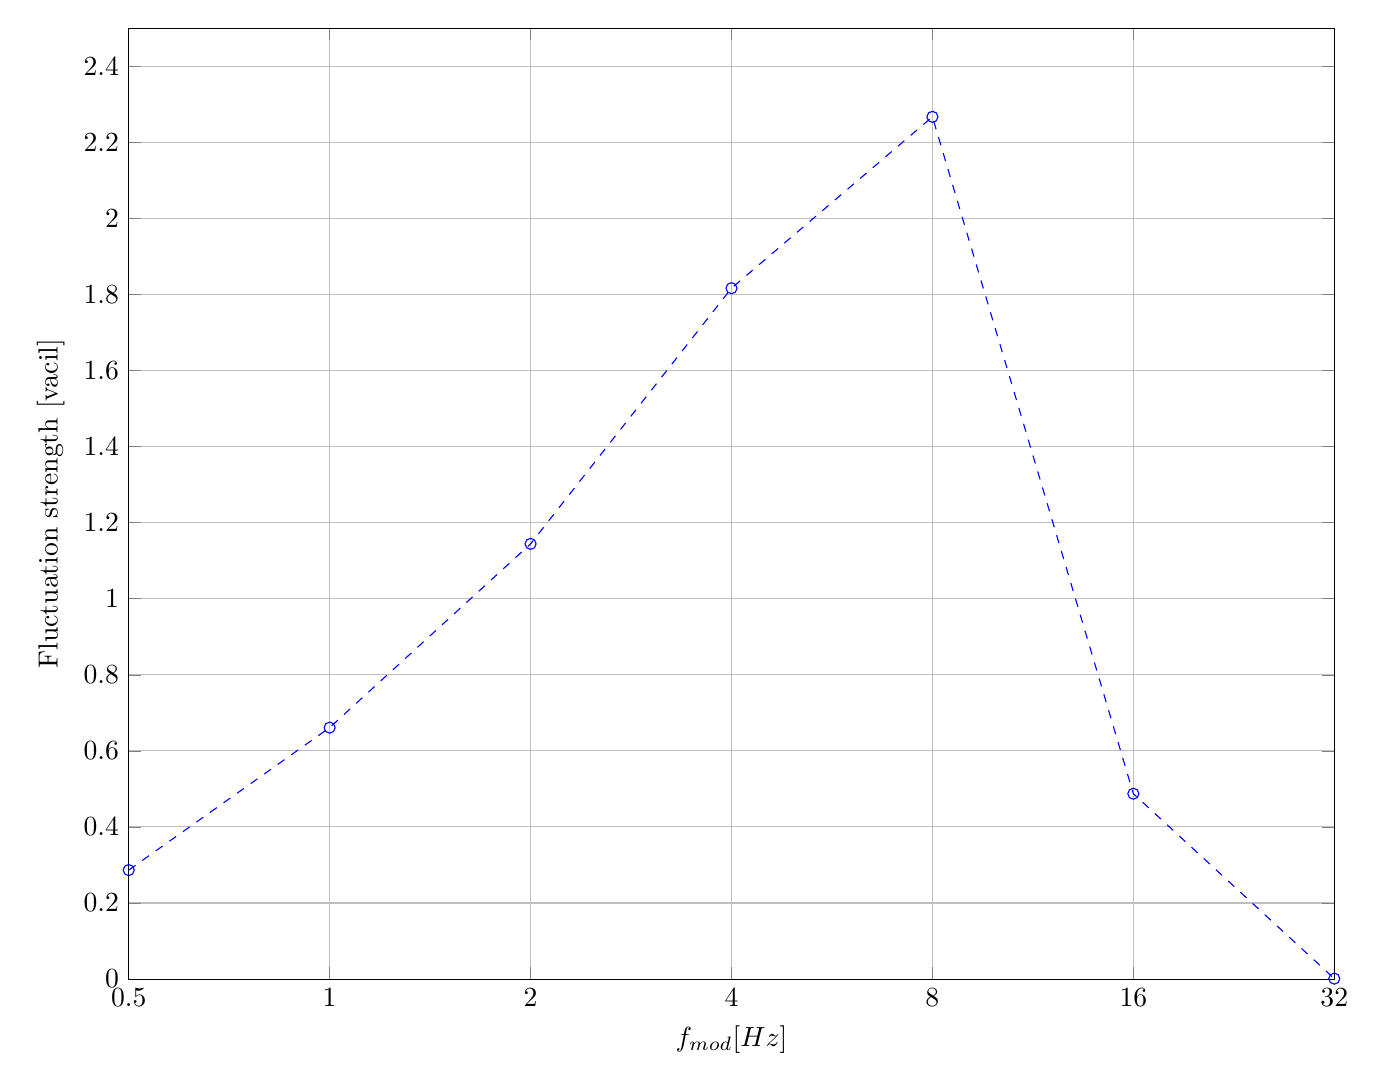
\begin{tikzpicture}

\begin{axis}[%
width=6.027778in,
height=4.754167in,
at={(1.011111in,0.641667in)},
scale only axis,
xmin=-1,
xmax=5,
xtick={-1,0,1,2,3,4,5},
xticklabels={{0.5},{1},{2},{4},{8},{16},{32}},
xlabel={$\text{f}_{\text{mod}}\text{ [Hz]}$},
xmajorgrids,
ymin=0,
ymax=2.5,
ylabel={Fluctuation strength [vacil]},
ymajorgrids
]
\addplot [color=blue,dashed,mark=o,mark options={solid},forget plot]
  table[row sep=crcr]{%
-1	0.286555303068175\\
0	0.661025694658725\\
1	1.14418319906766\\
2	1.81643964484805\\
3	2.26701825939723\\
4	0.487343827769812\\
5	0.00112052034248757\\
};
\end{axis}
\end{tikzpicture}%
    }
    \caption{Fluctuation strength as a function of modulation frequency for FM
        tones with $f_c = 1.5$ kHz, $d_f = 700$ Hz, SPL $= 70$ dB}
    \label{fig:FMtonesfmplot}
\end{figure}

\subsubsection{Carrier Frequency}

Figure \ref{fig:FMtonesfcplot} shows the relation between fluctuation strength
and carrier frequency, as estimated by the model.

\begin{figure}[ht]
    \centering
    \resizebox{!}{8cm}{
        % This file was created by matlab2tikz.
% Minimal pgfplots version: 1.3
%
%The latest updates can be retrieved from
%  http://www.mathworks.com/matlabcentral/fileexchange/22022-matlab2tikz
%where you can also make suggestions and rate matlab2tikz.
%
\begin{tikzpicture}

\begin{axis}[%
width=6.027778in,
height=4.754167in,
at={(1.011111in,0.641667in)},
scale only axis,
xmin=-1,
xmax=3,
xtick={-1,0,1,2,3},
xticklabels={{0.5},{1},{2},{4},{8}},
xlabel={$\text{f}_{\text{c}}\text{ [kHz]}$},
xmajorgrids,
ymin=0,
ymax=1.6,
ylabel={Fluctuation strength [vacil]},
ymajorgrids
]
\addplot [color=blue,dashed,mark=o,mark options={solid},forget plot]
  table[row sep=crcr]{%
-1	1.28501204791726\\
0	1.50837284117062\\
0.584962500721156	1.4183390265821\\
1	1.06180411560186\\
1.58496250072116	0.545973404320468\\
2	0.322553819275727\\
2.58496250072116	0.100526729779278\\
3	0.0465078546205861\\
};
\end{axis}
\end{tikzpicture}%
    }
    \caption{Fluctuation strength as a function of carrier frequency for FM
        tones with $f_m = 4$ Hz, $d_f = 700$ Hz, SPL $= 70$ dB}
    \label{fig:FMtonesfcplot}
\end{figure}

\subsubsection{Sound Pressure Level}

Figure \ref{fig:FMtonesSPLplot} shows the relation between fluctuation strength
and sound pressure level, as estimated by the model.

\begin{figure}[ht]
    \centering
    \resizebox{!}{8cm}{
        % This file was created by matlab2tikz.
% Minimal pgfplots version: 1.3
%
%The latest updates can be retrieved from
%  http://www.mathworks.com/matlabcentral/fileexchange/22022-matlab2tikz
%where you can also make suggestions and rate matlab2tikz.
%
\begin{tikzpicture}

\begin{axis}[%
width=6.027778in,
height=4.754167in,
at={(1.011111in,0.641667in)},
scale only axis,
xmin=40,
xmax=80,
xtick={40, 50, 60, 70, 80},
xlabel={SPL [dB]},
xmajorgrids,
ymin=0.4,
ymax=2.4,
ylabel={Fluctuation strength [vacil]},
ymajorgrids
]
\addplot [color=blue,dashed,mark=o,mark options={solid},forget plot]
  table[row sep=crcr]{%
40	0.598381292724765\\
50	1.09078652252618\\
60	1.46262386637619\\
70	1.81643964406686\\
80	2.3505389064298\\
};
\end{axis}
\end{tikzpicture}%
    }
    \caption{Fluctuation strength as a function of sound pressure level for FM
        tones with $f_c = 1.5$ kHz, $f_m = 4$ Hz, $d_f = 700$ Hz}
    \label{fig:AMtonesSPLplot}
\end{figure}

\subsubsection{Frequency Deviation}

Figure \ref{fig:FMtonesdfplot} shows the relation between fluctuation strength
and frequency deviation, as estimated by the model.

\begin{figure}[ht]
    \centering
    \resizebox{!}{8cm}{
        % This file was created by matlab2tikz.
% Minimal pgfplots version: 1.3
%
%The latest updates can be retrieved from
%  http://www.mathworks.com/matlabcentral/fileexchange/22022-matlab2tikz
%where you can also make suggestions and rate matlab2tikz.
%
\begin{tikzpicture}

\begin{axis}[%
width=6.027778in,
height=4.754167in,
at={(1.011111in,0.641667in)},
scale only axis,
xmin=0,
xmax=700,
xlabel={$\text{d}_{\text{f}}\text{ [Hz]}$},
ymin=0,
ymax=2,
ylabel={Fluctuation strength [vacil]}
]
\addplot [color=blue,dashed,mark=o,mark options={solid},forget plot]
  table[row sep=crcr]{%
16	0.0136678989035672\\
32	0.0667765982600906\\
100	0.681767637001039\\
300	1.44923619591073\\
700	1.81643964484805\\
};
\end{axis}
\end{tikzpicture}%
    }
    \caption{Fluctuation strength as a function of deviation frequency for FM
        tones with $f_c = 1.5$ kHz, $f_m = 4$ Hz, $SPL = 70$ dB}
    \label{fig:FMtonesdfplot}
\end{figure}

\end{document}
